\subsection{Difference Image Analysis: Transience and Variable Objects}
\label{sec:dia_transient_variable}


\subsubsection{DIA Status}

As we have started to obtain repeated science-quality images of some fields, we have begun to build coadded templates as part of the regular weekly cumulative Data Release Processings. 
These mini-DRPs also include difference image analysis (DIA) of their constituent exposures.
Using the DRP-produced templates, we have also obtained near-real-time difference images in Prompt Processing for a few exposures. 
We have not yet had the opportunity to begin tuning template generation, difference imaging, or Real/Bogus characterization of these data, so the report below provides an initial rough characterization of DIA performance. 

\subsubsection{ML Reliability and Artifact Rates}

We ran a convolutional neural network on 51$\times$51 difference, science, and template cutouts for 912k DIASources identified in the \texttt{w\_2024\_47} data release processing.  
This processing primarily includes data from extragalactic deep fields.
These DiaSources were obtained from 4252 detector-visit images, implying an average of 21 DIASources per detector or about four thousand per equivalent full LSST focal plane.
This is somewhat less than the ten thousand DIASources expected per visit and may reflect lower sensitivity due to ongoing image quality refinement and early templates.

The CNN was trained on simulated DC2 images with additional point source injection, so caution is needed when interpreting the values returned by this classifier on ComCam data.
Nevertheless,  Figure \ref{fig:reliability_hist} shows a clear separation in reliability scores and would imply roughly a 3:1 bogus:real ratio if taken at face value.
These values will be confirmed with manual inspection.
We plan to train a purpose-built classifier on larger samples of labeled ComCam data.

\begin{figure}
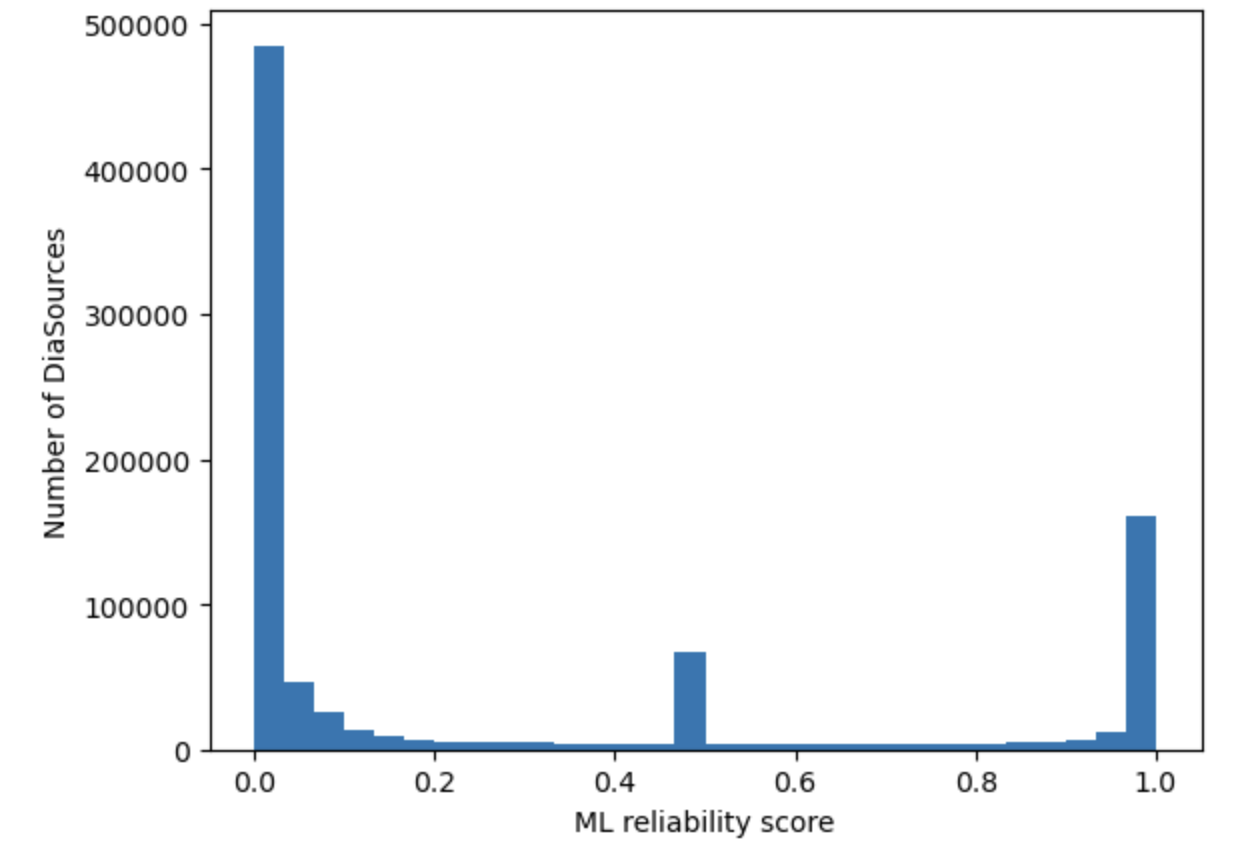
\includegraphics[width=\textwidth]{dia/figures/reliability_histogram.png}
\caption{Histogram of machine-learned reliability scores computed on ComCam difference images. \label{fig:reliability_hist}}
\end{figure}

\subsection{Difference imaging QA}

\begin{figure}
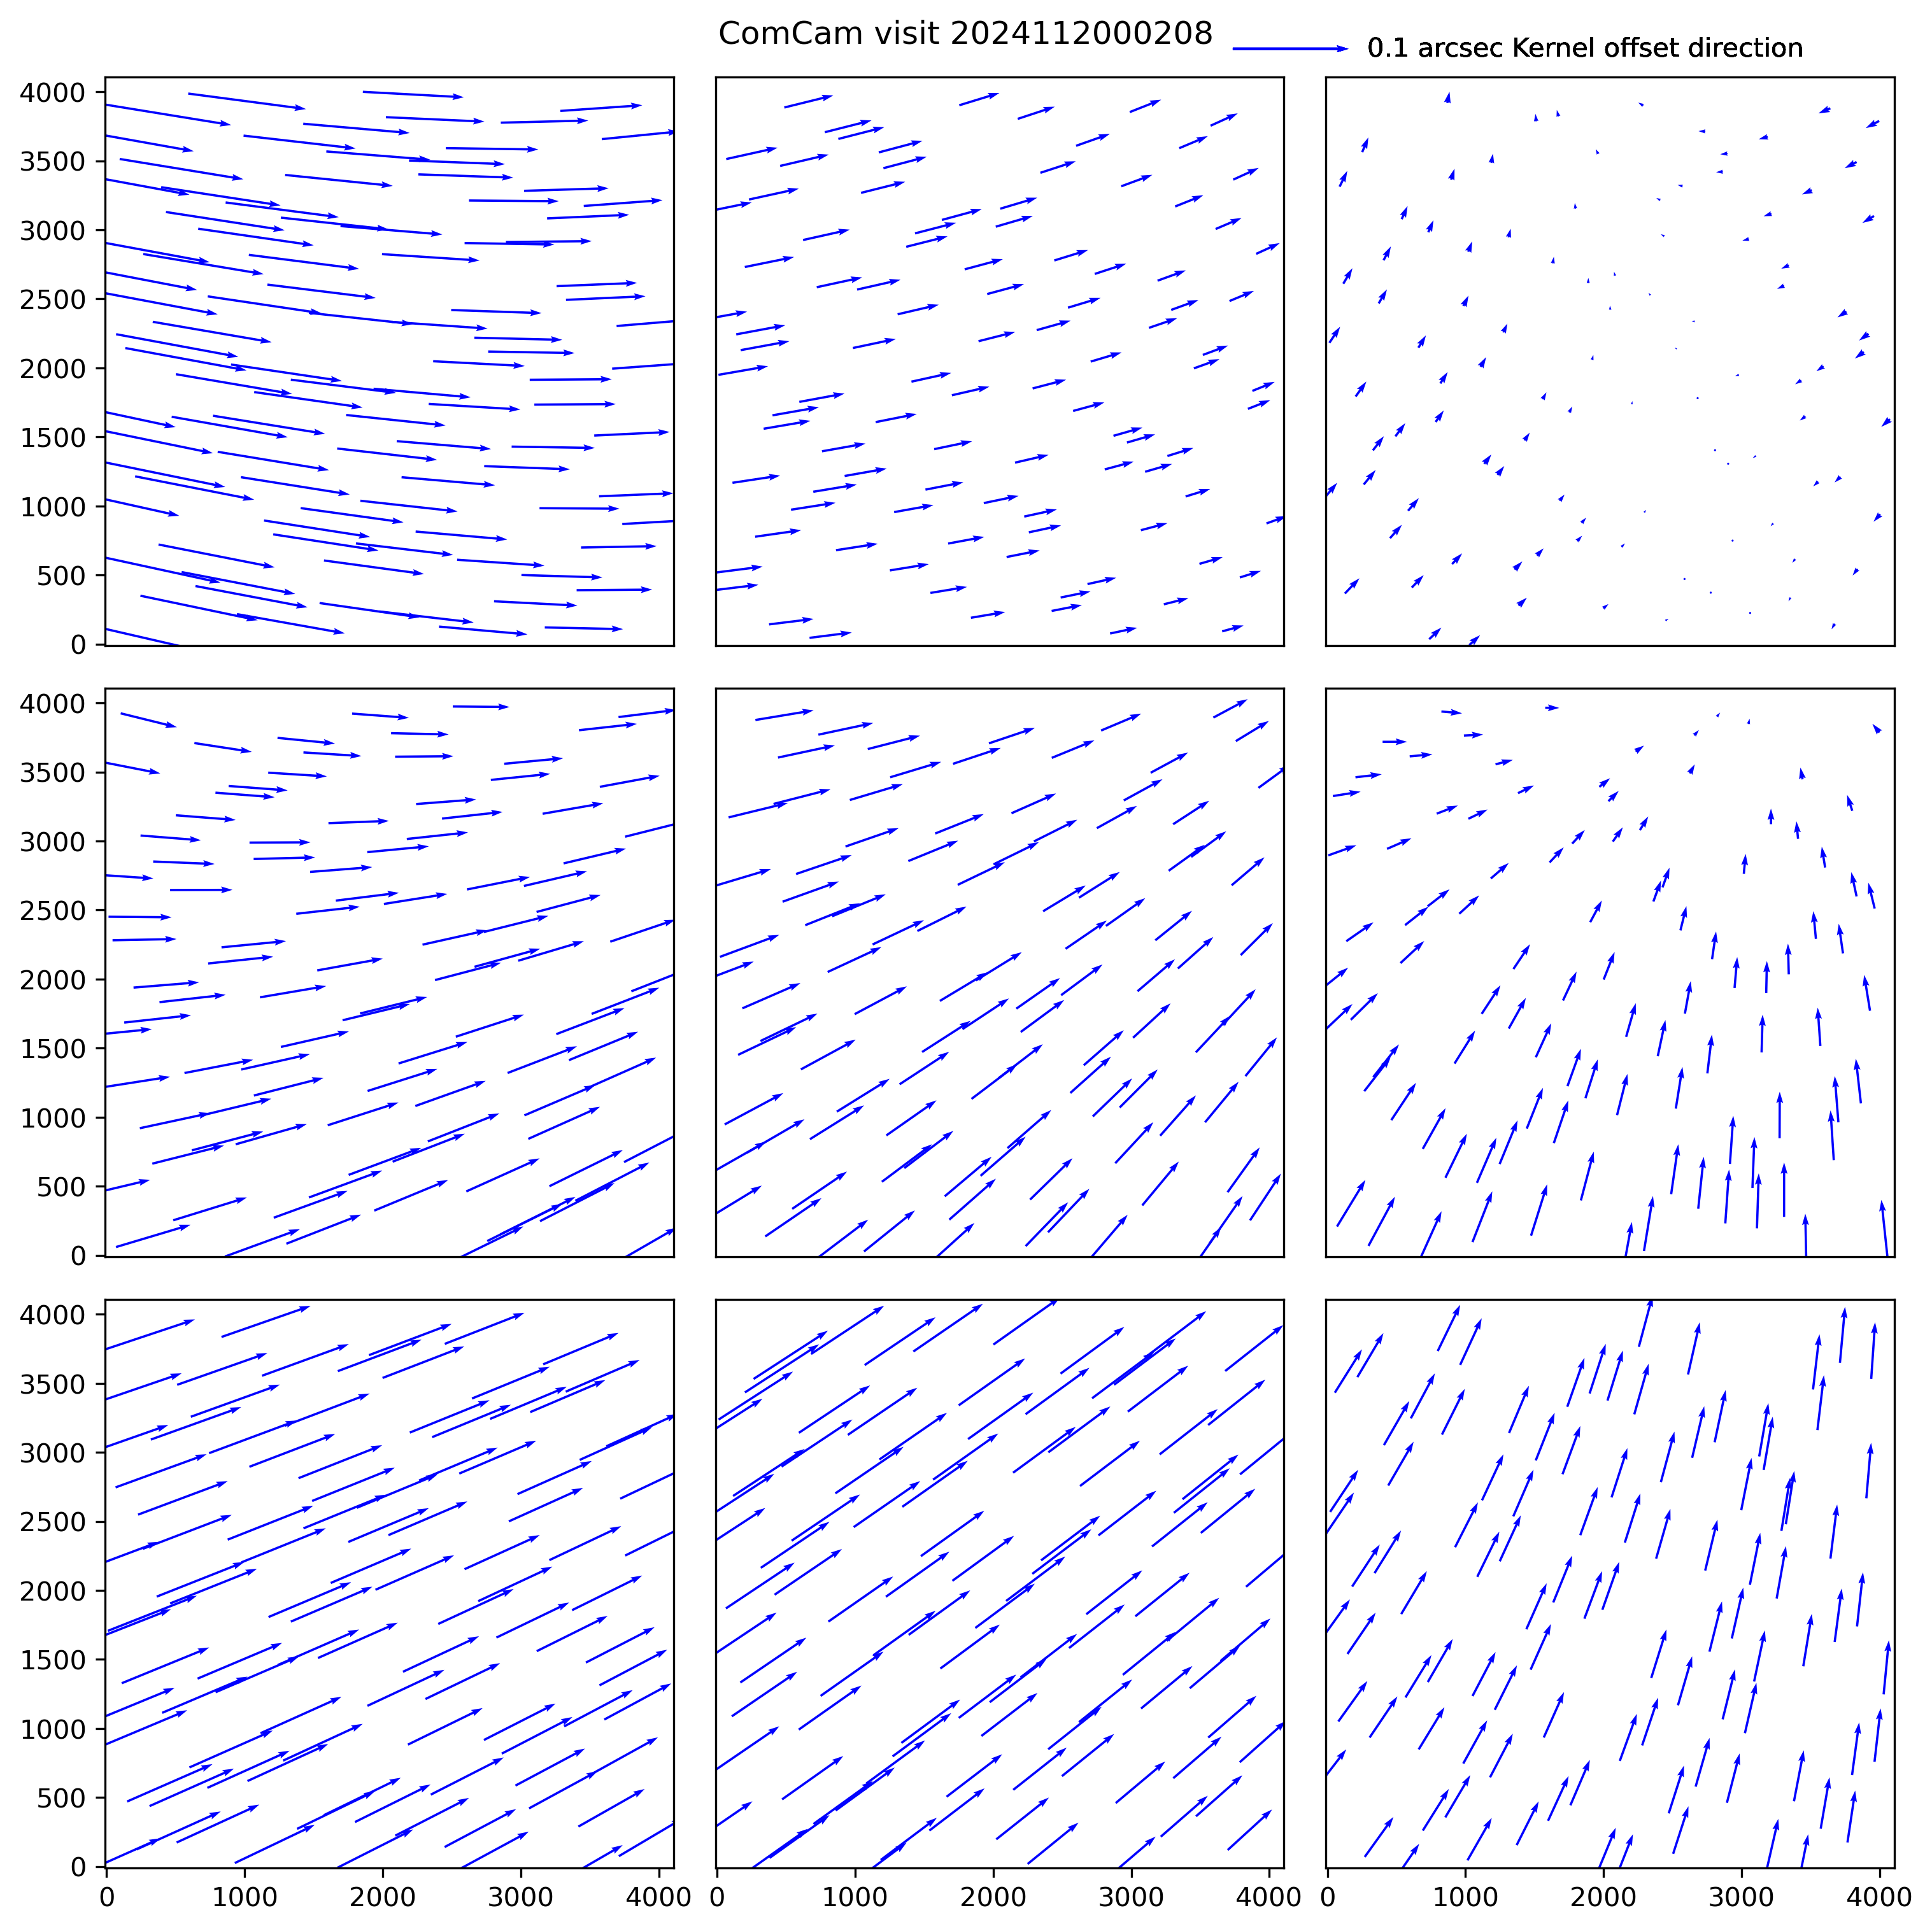
\includegraphics[width=\textwidth]{dia/figures/ComCam_kernel_quiver_2024112000208.png}
\caption{Quiver plot of the implied offset between the science and template images,
  calculated from the centroid of the PSF matching kernel.
  Note that the scale differs between the different panels, but that the overall pattern
  appears coherent over the focal plane, although each CCD was solved independently.
  \label{fig:diffim-quiver}}
\end{figure}

A difference imaging afterburner is run manually on Prompt Processing output to generate diagnostic plots, such as \ref{fig:diffim-quiver}.
From \ref{fig:diffim-quiver} we see the centroid of the PSF matching kernel sampled across one detector, which reveals a systematic offset between the science and template images.
A similar offset is seen across the rest of the detectors for this visit, and in other visits.
The images comprising the template used the same astrometric reference catalog as the science image in this case, but the template was constructed with the calibrate+characterizeImage pipeline while the science image was processed with calibrateImage.
These are not included in the Prompt Processing payload to save critical time during observing.

The distribution of sources detected on the difference image reveals some detector-level effects that are not fully accounted for.
Binning the locations of the diaSources in 1-D in \ref{fig:diaSource-distribution} by their x- and y-values reveals systematic overdensities of detections at the amplifier boundaries in x (but not in y).
Additional overdensities seen in y-band may be from the residual phosphorescent wax reported to be left on some chips beneath the AR coating.

\begin{figure}
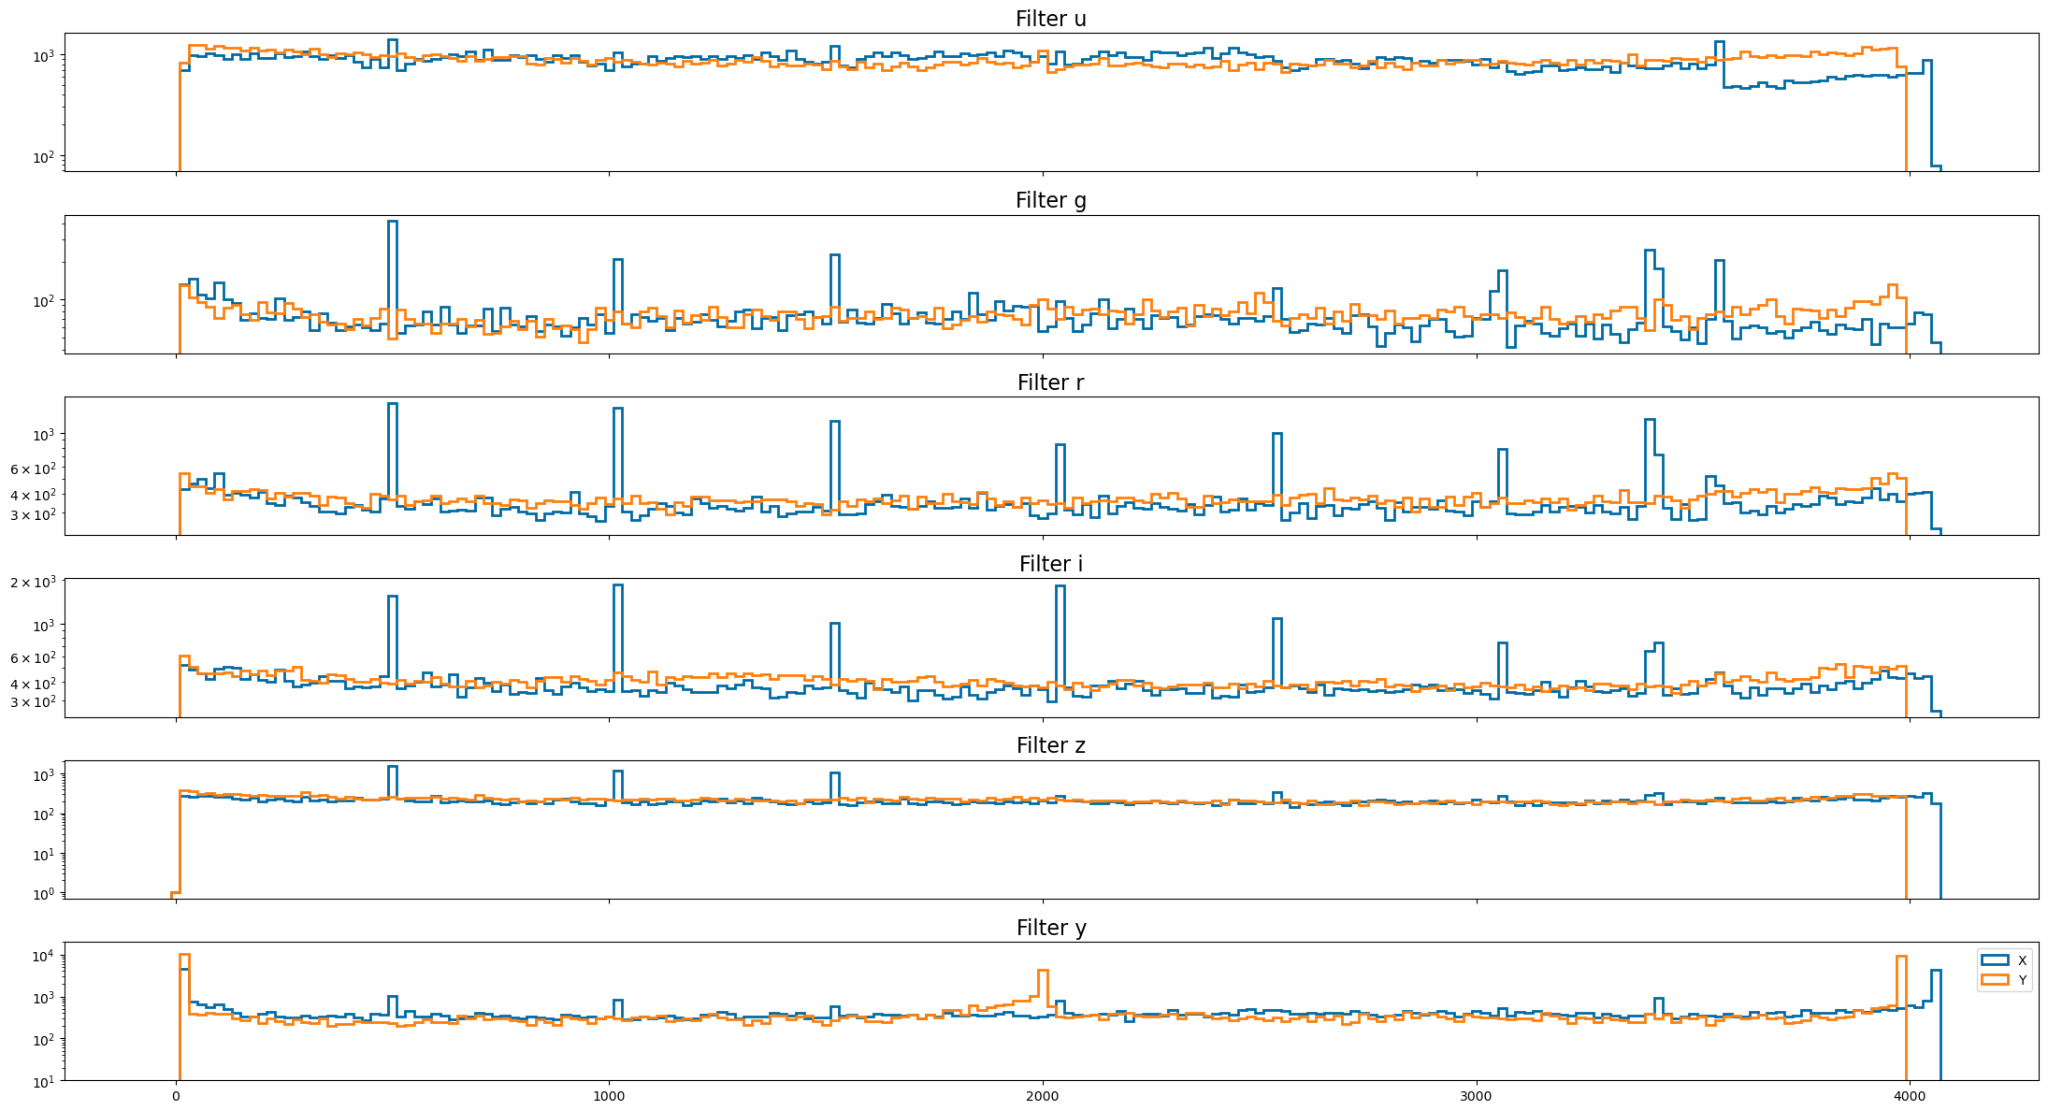
\includegraphics[width=\textwidth]{dia/figures/diaSource_distribution.png}
\caption{Binning the locations of the diaSources in 1-D by their x- and y-values reveals systematic overdensities of detections at the amplifier boundaries in x (but not in y). \label{fig:diaSource-distribution}}
\end{figure}

\iffalse                                % doesn't analyse comCam data.
\subsection{Cosmic Ray Detection Performance}

In this analysis, we evaluate the performance of the cosmic ray detection algorithm by integrating real cosmic ray events into simulated observational data and applying standard detection pipelines to assess their performance. The primary objective is to assess the algorithm's ability to accurately identify cosmic rays, thereby ensuring data purity for subsequent scientific analyses.

\subsubsection{Methodology}

We used 67 visits (603 detectors), where the dark frames were taken from 2024-10-27 to 2024-11-01, and the simulated exposures are from $day\_obs=20240626$.

We processed a set of simulated on-sky images from the ComCamSim OR4 repository and added real ComCam dark frames containing only cosmic rays. First, we performed Instrument Signature Removal (ISR) on ComCam darks as well as ComCamSim separately. After that, we combined the two images and performed image characterization and calibration.

To establish ground truth, we used the ComCam dark frames and identified pixels that were brighter than 5 times the standard deviation above the mean background level. This threshold allowed us to create a ground truth mask representing cosmic rays. At the end of the process, we compared this ground truth mask with the cosmic ray (CR) mask obtained after the characterization step to evaluate the algorithm's performance.

\subsubsection{Results}

The detection outcomes were categorized into four classes: True Positives (TP), False Positives (FP), True Negatives (TN), and False Negatives (FN). The counts for each category are presented in Table~\ref{tab:confusion_matrix}. The True Positives, False Positives, True Negatives, and False Negatives represent the comparison between the CR mask and the ground truth mask. Critical False Negatives (CFN), on the other hand, are the pixels that are considered detections (from the DETECTED mask) but are, in fact, cosmic rays.

\begin{table}[H]
    \centering
    \caption{Confusion Matrix for Cosmic Ray Detection (Pixel counts)}
    \label{tab:confusion_matrix}
    \begin{tabular}{*3c}
        \hline
        & \textbf{Positive (Detected)} & \textbf{Negative (Not Detected)} \\
        \hline
        \textbf{True (Cosmic Ray)}  & 223,982 & 92,366 \\
        \textbf{False (Non-Cosmic Ray)} & 86,094  & 9,821,261,558 \\
        \hline
         \multicolumn{2}{c}{\textbf{CFN (Cosmic Ray detected as Source)}} & 27954 \\
    \end{tabular}
\end{table}

From these results, we calculated the following performance metrics:

\begin{itemize}
    \item \textbf{Purity (Precision):} 
    \begin{equation*}
        \text{Purity} = \frac{TP}{TP + FP} = \frac{223,982}{223,982 + 86,094} \approx 0.722
    \end{equation*}
    \item \textbf{Completeness (Recall):} 
    \begin{equation*}
        \text{Completeness} = \frac{TP}{TP + FN} = \frac{223,982}{223,982 + 92,366} \approx 0.708
    \end{equation*}
    \item \textbf{Adjusted Completeness:} Considering critical false negatives (CFN), where cosmic rays were detected as sources, the adjusted completeness is 
    \begin{equation*}
        \text{Adjusted Completeness} = \frac{TP}{TP + CFN} = \frac{223,982}{223,982 + 27,954} \approx 0.889
    \end{equation*}
\end{itemize}

\subsubsection{Discussion}

The results indicate that the current cosmic ray detection algorithm demonstrates moderate success in identifying cosmic rays, as evidenced by a purity of approximately 72.2\%. This suggests that most of the detections are indeed true cosmic rays, though a significant portion, about 27.8\%, are false positives.

The completeness, at around 70.8\%, reveals that while the algorithm is capable of detecting a majority of cosmic rays, it still misses a substantial number of events. However, the adjusted completeness of 88.9\% highlights the algorithm's improved performance when considering critical false negatives—those cosmic rays that were detected but mistakenly classified as sources rather than cosmic rays. 


\fi

\subsection{Satellite Streaks}

As orbital space becomes increasingly crowded, we expect to see many bright streaks, flares, and glints due to satellites and other reflective human-made objects orbiting the Earth. The majority of the population is in low-Earth orbit (LEO). For a review of the current status and likely impacts to LSST, please see \url{ls.st/satcon}.

As expected, many ComCam detector-visit images clearly show streaks. Visual inspection of nearly all ComCam images to date are being recorded on a best-effort basis in a Confluence Database dubbed ``ComCam Satellite Spotter,'' and as of 2024 Nov 25 there are over 500 rows. The simple schema has one row per visit (if a streak crosses multiple detectors --- which it often does --- this is indicated in the ``detector'' column). In general, the morphology of streaks falls into one of these categories:
\begin{itemize}
\item Straight bright linear feature, typically at least 20 pixels wide, that crosses one or more detectors and goes off the edge (typical of most LEO satellites, such as Starlink)
\item Shorter version of the above, with clear start and/or endpoints, which usually indicates the object imaged is located at a higher-than-LEO orbital altitude (and/or the exposure integration time was unusually short)
\item Intermittent linear feature, i.e., a dashed line, due to different parts of the satellite having different reflective properties
\item A flare or glint brightening event that fades in and out along a linear trajectory, either isolated or as part of a longer streak
\item Actually a bright star diffraction spike
\item Actually a cosmic ray that was not repaired
\item Variation of any of the above but in out-of-focus donut form (interestingly, depending on altitude, certain streaks may appear either in- or out-of-focus when stars appear as donuts)
\end{itemize}

Thanks to ComCam's relatively small field of view and the satellite population being as small as it ever will be during Rubin Commissioning and Operations, we have not yet seen an overwhelmingly bright satellite (e.g., BlueWalker 3 or one of the BlueBirds, all operated by AST SpaceMobile). Only a couple instances have streaks bright enough to induce visually-obvious crosstalk ``secondary streaks;'' the majority of streaks are relatively faint and the only portion of the image impacted are regions overlapping with the streak itself on the sky. Reliably determining streak width is an ongoing challenge, as it is not a delta function, and some of the brighter streaks do have notably extended stray light profile wings.

We note the Science Pipelines' algorithmic approach to identifying linear streak features  (see \url{https://dmtn-197.lsst.io}) uses the detected mask plane and not the image array (pixel values) for efficiency. To more effectively detect faint streaks in difference images, as in the DECam example shown in Figure \ref{fig:decam-streak}, we have recently implemented a binning scheme designed to be sensitive to linear features that fall below the detection threshold.

\begin{figure}[ht!]
    \centering
    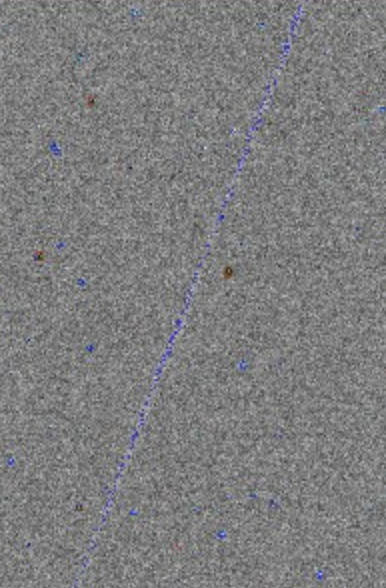
\includegraphics[width=0.5\linewidth]{figures/decam-streak.png}
    \caption{THIS IS DECAM, NOT COMCAM. A typical faint satellite streak in a portion of a difference image where only some regions in the streak fall above the image detection threshold. The streak detection algorithm did not recognize this as a streak, because the regions of the image masked detected (blue) are not contiguous. After binning the image to effectively boost the streak surface brightness, it was readily detected.}
    \label{fig:decam-streak}
\end{figure}

\subsubsection{Mitigating streaks in DRP}

In most situations, the usual outlier clipping done during coadd assembly with the CompareWarp algorithm excludes streaks from coadds. The coadds where streaks remain all tend to have very few input images, so the streak was not able to be flagged and excluded as an outlier. Work is underway to assess the performance of detecting streaks via the kernel Hough transform in ComCam on top of the standard outlier clipping.

\subsubsection{Mitigating streaks in AP}

Work is underway to detect and masking streaks and glints in difference images. ComCam observations are an important data set for testing how well this works in various situations. A more detailed report will be available in the coming weeks. The efforts described here are distinct from work to identify long trailed sources and cross-check with an external satellite catalog.

\subsubsection{Additional streak considerations}

A streak showed up in an i-band flat and was used to make a combined flat, so a few visit images processed with this flat had an erroneous dark streaks. This was easily resolved by excluding the problematic flat exposure, but it was a manual process to notice the problem.

It is possible to use public satellite catalog data to ID some satellites, which will be useful for providing feedback to satellite operators and others to measure how the changing satellite population is affecting science and the sky over the course of LSST. A preliminary field-of-view query service is available via IAU CPS SatChecker (see \url{https://satchecker.readthedocs.io/en/latest/}).

Before LSST begins in earnest, it will be necessary to coordinate with the Scheduler team to proactively avoid the brightest satellites.


\subsection{Fake Source Injection for DIA}
\subsubsection{Selection of a data subset}

We selected a subset of 24 visits chosen from observations processed by the DRP pipelines that included image
subtraction, in order to learn about DIA performance, as well as that of the detection and measurement
algorithms.

We chose visits with a zenith distance of less than 45 degrees, as well as some technical parameters, derived from the nominal DRP DIA performance (ratio of PSF between template and science, as well as Kernel basis condition number). 

We create a catalog of fakes for these visits by injecting synthetic sources near true sources which are
possibly extended, and with a flux within 1.5 magnitudes of the selected source host
(\figRef{scatter_radec_diaSrcs_match_arsec_mag})

\begin{figure}
    \centering
    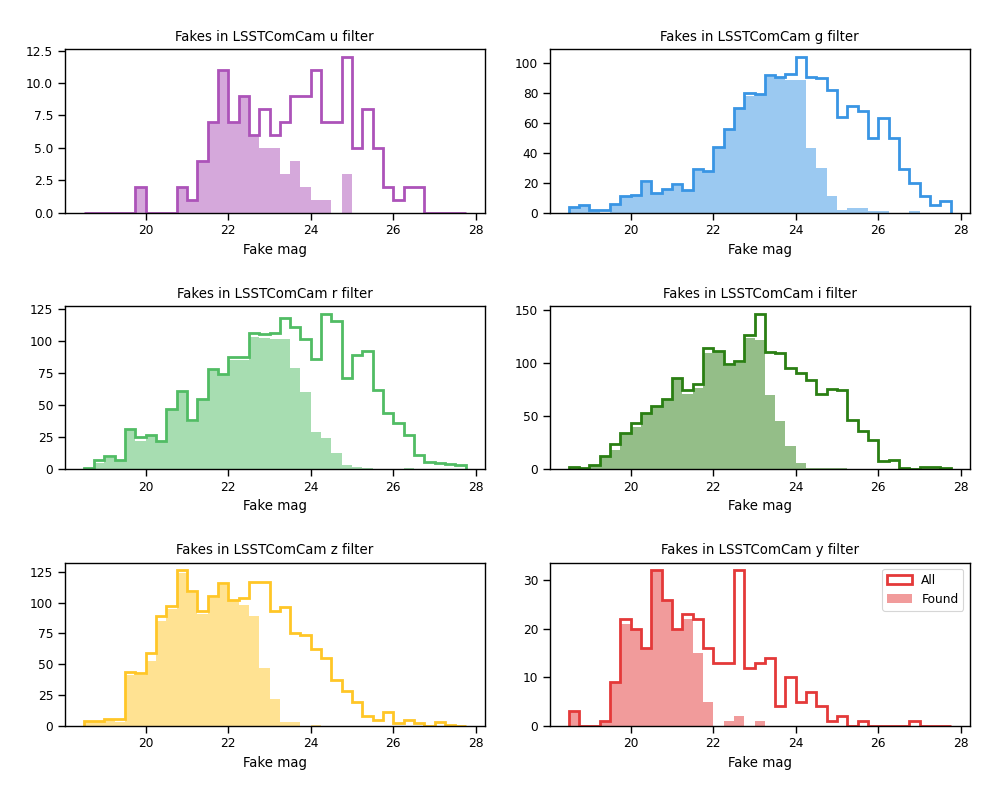
\includegraphics[width=0.5\linewidth]{dia/figures/simple_hist_completeness_mag_per_filter.png}
    \caption{The distribution of magnitudes per bandpass for all the injected fakes (solid lines), and in shaded region the distribution of magnitudes of the fakes detected by the AP pipeline.}
    \label{fig:found_fakes_per_Filter}
\end{figure}


We run Alert Production pipeline with a set of additional tasks that handle fake injection on the
\texttt{initial\_pvi} images, and then the book-keeping tasks of fake catalog matching to diaSources as well
as forced photometry for SNR estimation. We then cross-matched the position of our candidate detections, or
\textit{diaSources} with the positions of the synthetic sources, using a tolerance of $0.5''$ (roughly
$2.5$px).

Those fakes that found a match are called ``found fake'' and objects that had no match we refer as ``lost'' or
``missed'' fakes.  The rate of found to existing fakes is our recovery rate, Recall or Efficiency of detection.

\begin{figure}
    \centering
    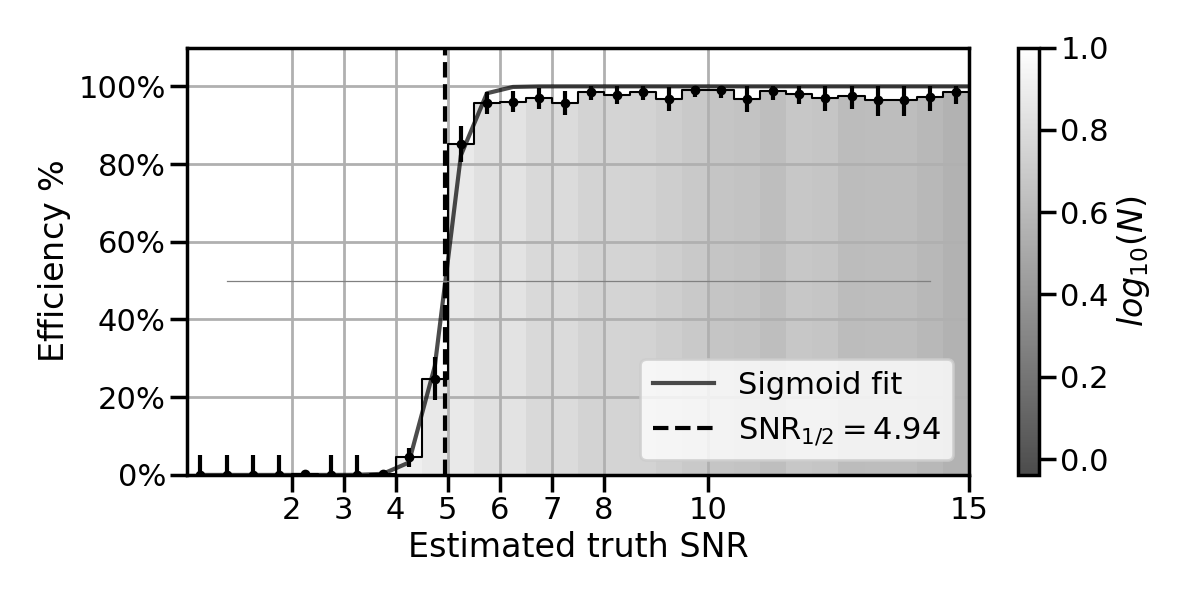
\includegraphics[width=0.95\linewidth]{dia/figures/Efficiency_vs_forced_base_PsfFlux_instFlux_SNR.png}
    \caption{The detection efficiency as function of the PSF estimated S/N ratio of the fake sources. The SNR 1/2 parameter is also included in dashed lines, and represents the 50\% efficiency S/N threshold value (lower is better).}
    \label{fig:eff_vs_snr_fakes}
\end{figure}

\begin{figure}
    \centering
    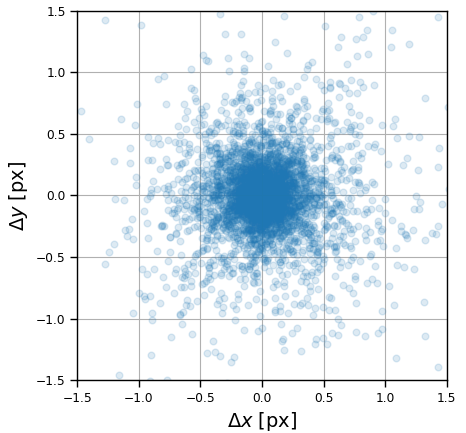
\includegraphics[height=0.3\textheight]{dia/figures/scatter_xy_diaSrcs_match_px.png}
    \hfil
    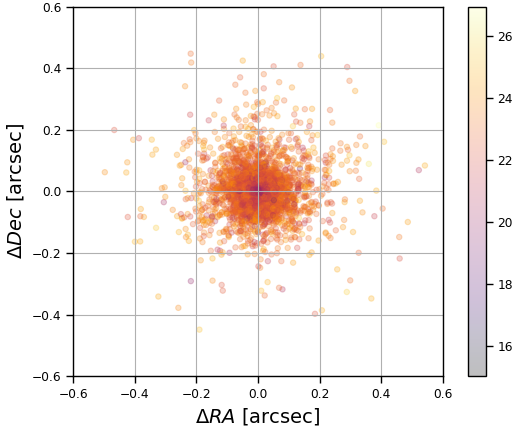
\includegraphics[height=0.3\textheight]{dia/figures/scatter_radec_diaSrcs_match_arsec_mag.png}
    \caption{The scatter of the coordinate centroid recovery of the fakes. In the left we have the scatter around the true centroid in pixel coordinates, and in the right the scatter around the true center of fakes in sky coordinates (and in units of arc-seconds), wit the grid matching the pixel grid by means of the platescale. Also, we include the brightness in colormap.}
    \label{fig:scatter_radec_diaSrcs_match_arsec_mag}
\end{figure}

\iffalse                                % doesn't add much to the PSF mags, and has more scatter
\begin{figure}
    \centering
    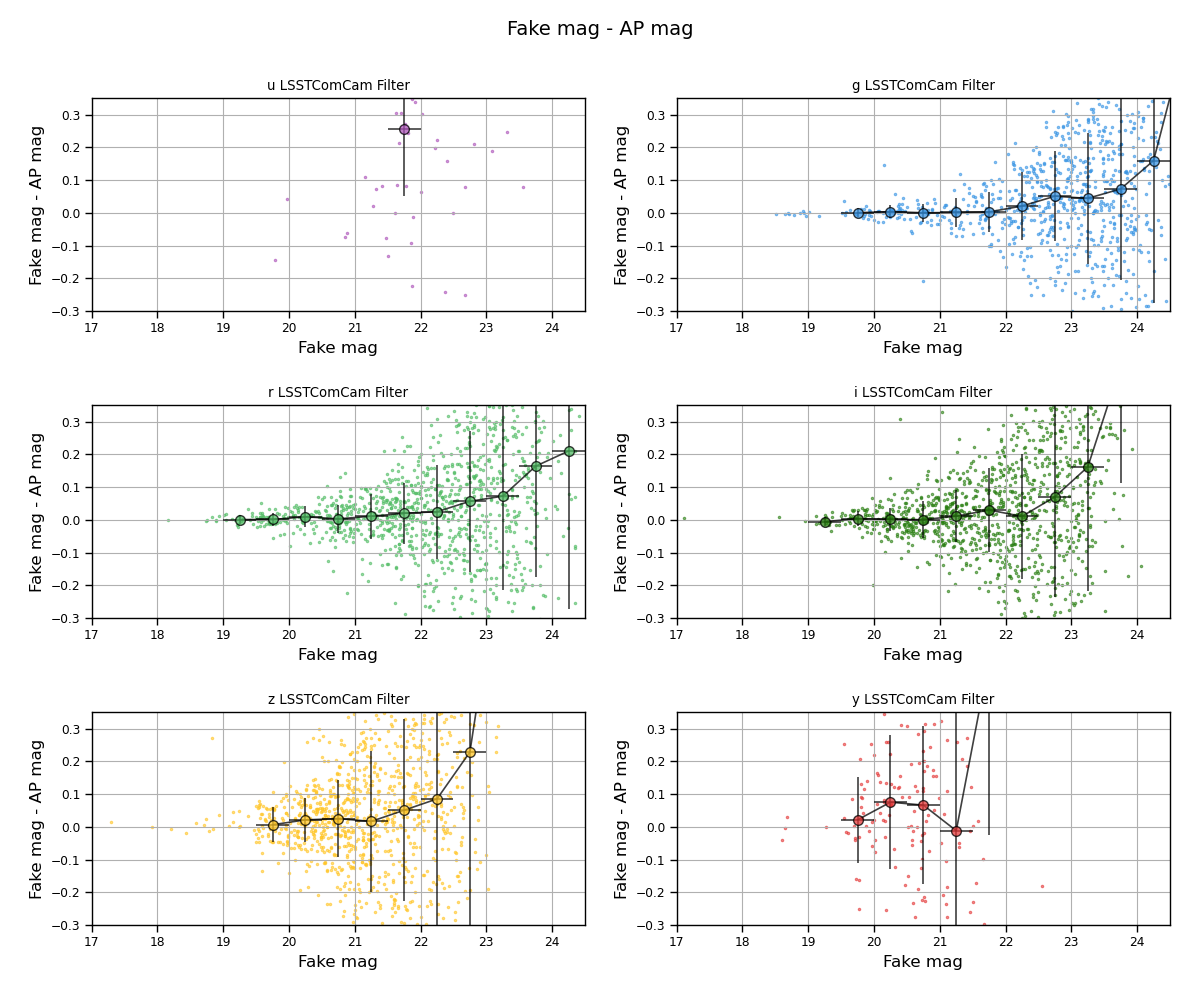
\includegraphics[width=0.95\linewidth]{dia/figures/scatter_mag_ap_mag_perfilter.png}
    \caption{The recovered Aperture magnitude residual per filter for all the found fake sample, as a function of their true magnitude. }
    \label{fig:photometric_recovery_vs_fakemag}
\end{figure}
\fi

\begin{figure}
    \centering
    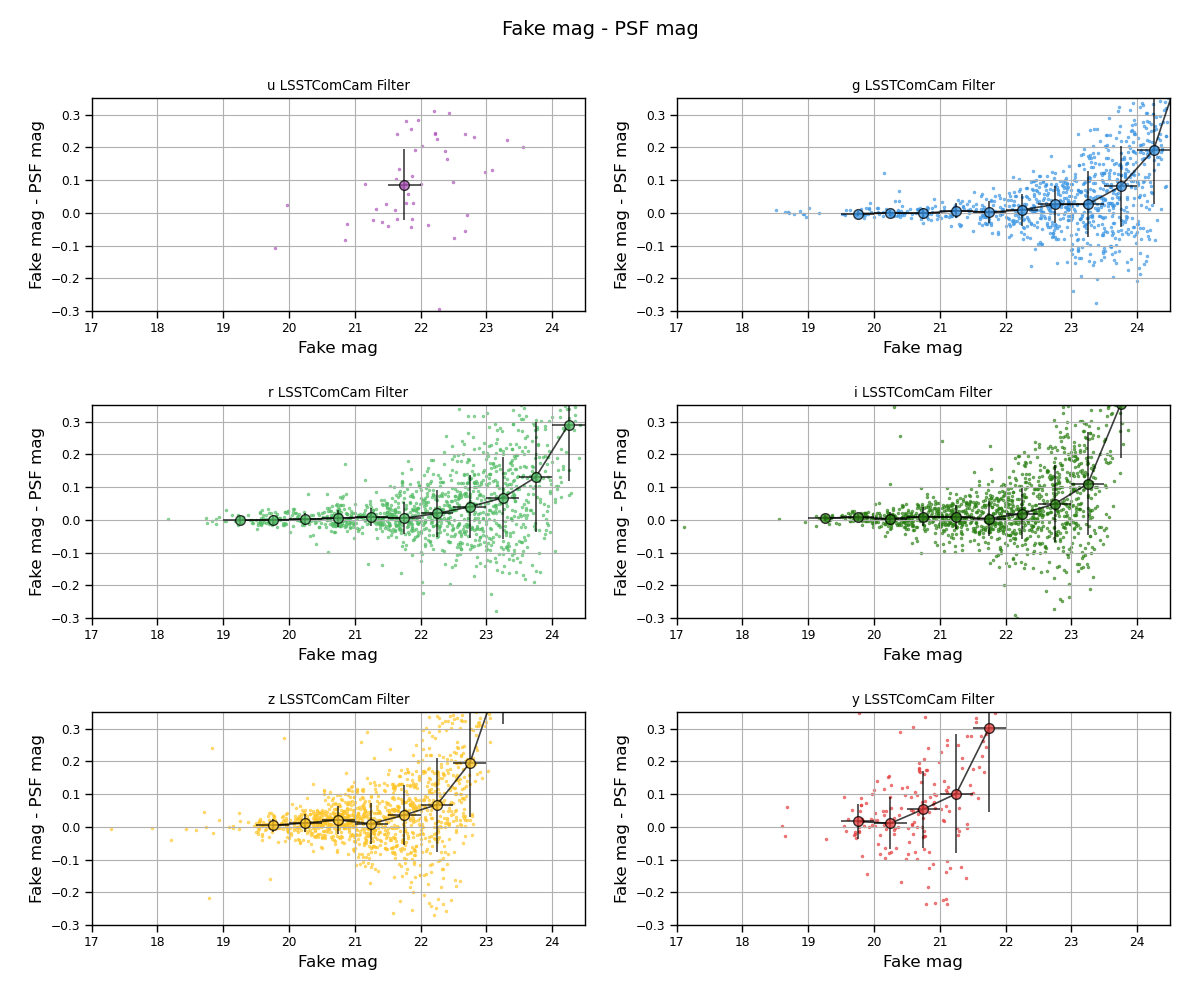
\includegraphics[width=0.45\textwidth]{dia/figures/scatter_mag_psf_mag_perfilter.png}
    \hfil
    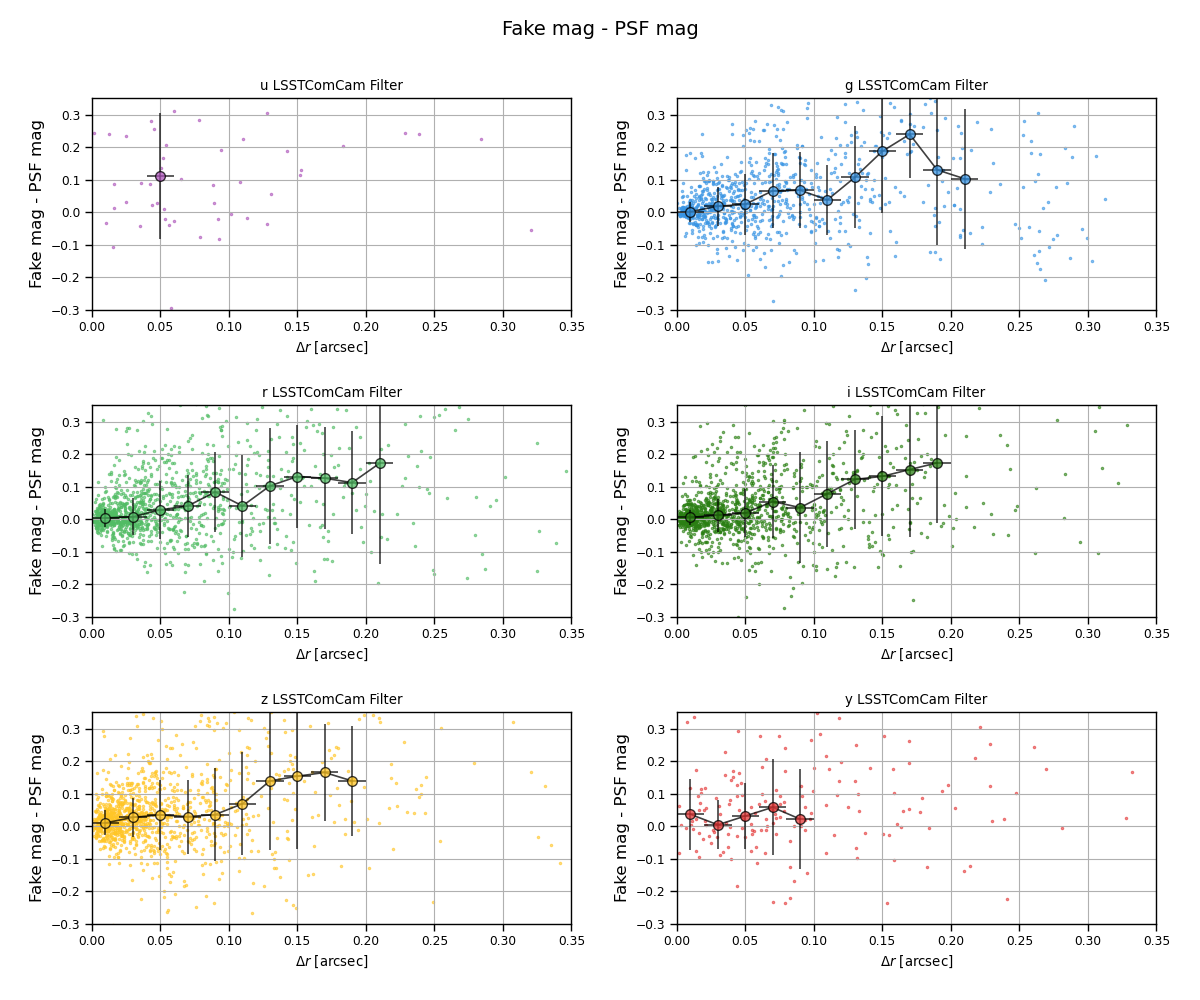
\includegraphics[width=0.45\textwidth]{dia/figures/scatter_dist_psf_mag_perfilter.png}
    \caption{The residual of PSF magnitude measurement for found fakes, as function of their true magnitude
    (left) or matching distance in arcsec (right).}
    \label{fig:dia_photometric_recovery}
\end{figure}

\iffalse                                % Needs to be analysed as a function of flux
\begin{figure}
    \centering
    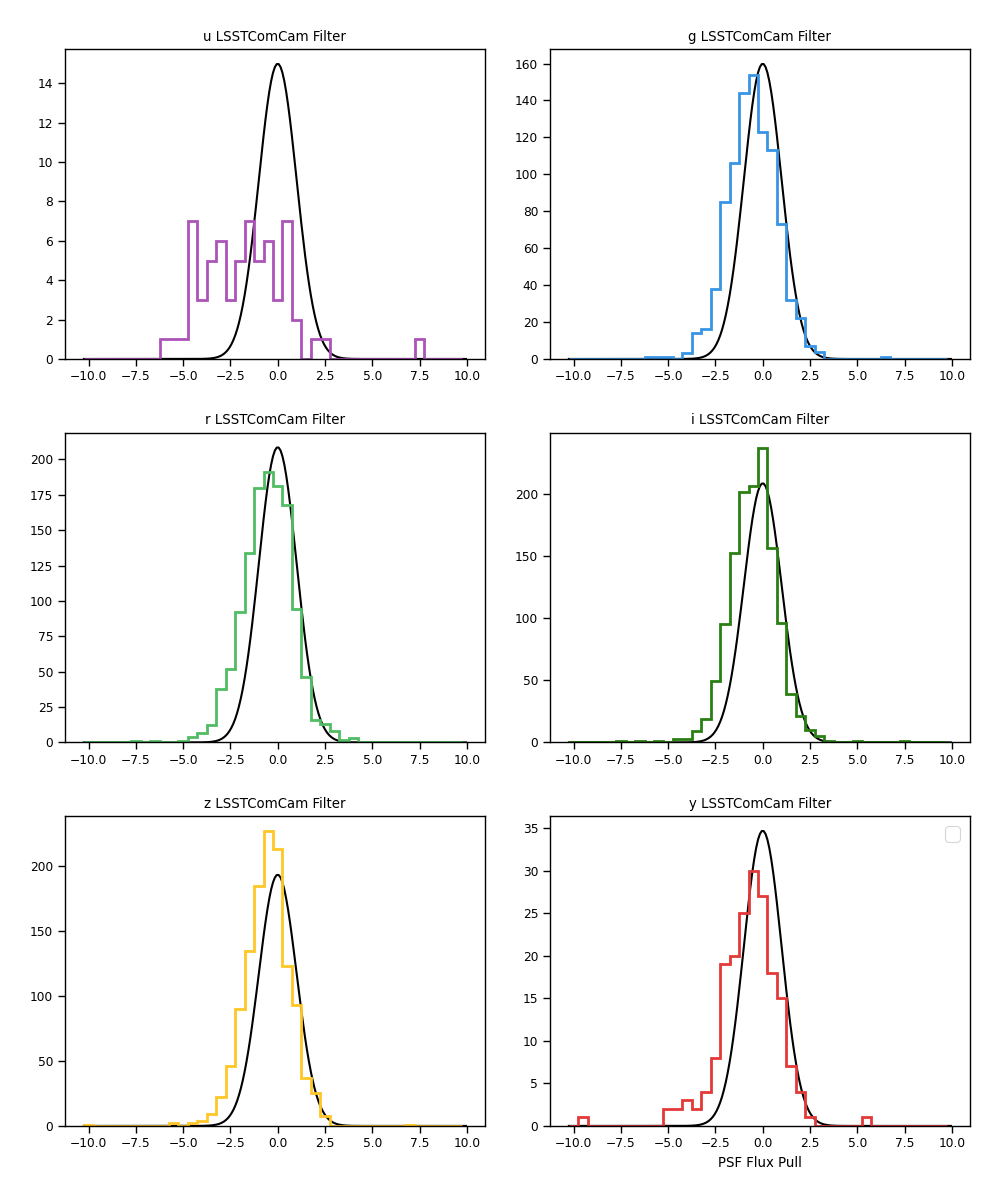
\includegraphics[width=0.95\linewidth]{dia/figures/flux_pulls.png}
    \caption{The flux pull (``$\chi$'') distribution for all the found fakes, in each filter bandpass. A zero mean, unit dispersion Gaussian distribution function is also included for reference.}
    \label{fig:fake_sources_pulls}
\end{figure}
\fi

\iffalse                                % what does this tell us?
\begin{figure}
    \centering
    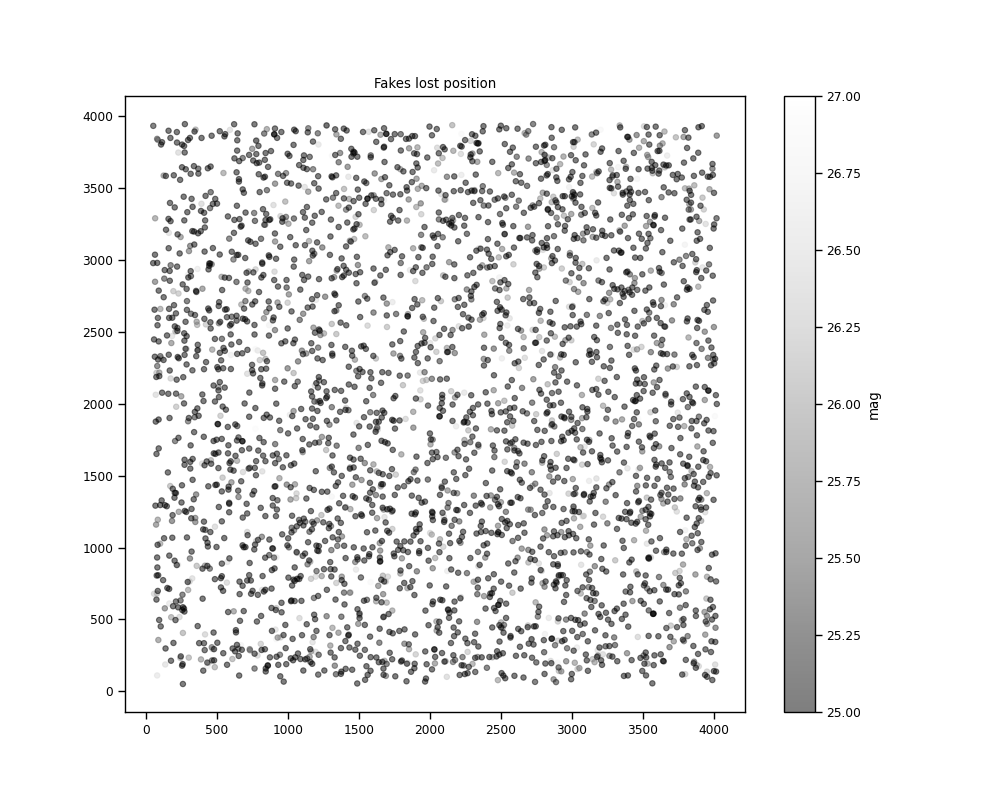
\includegraphics[width=0.95\linewidth]{dia/figures/lost_sources_detector_map.png}
    \caption{The scatter map of the lost sources in the detector coordinates. In gray scale in the colorbar we show the object magnitudes.}
    \label{fig:lost_sources_xy}
\end{figure}
\fi

The detection efficiency is plotted in \figRef{eff_vs_snr_fakes}; 
the astrometric errors in the recovered synthetic sources is shown in
\figRef{scatter_radec_diaSrcs_match_arsec_mag}, while the photometric errors appear
in \figRef{dia_photometric_recovery}



